\chapter{Verwendung der Vorlage}\label{cha:TemplateIntroduction}

Die Vorlage ACIN\_bac\_report.cls stellt eine Klasse zum Schreiben von
Bakkalaureats-Arbeiten zur Verf�gung.
Folgende Dateien werden ben�tigt:
\begin{itemize}
  \item \emph{ACIN\_bac\_report.cls} Die Klassendatei. Diese Datei sollte
  nicht ge�ndert werden.
  \item \emph{graphics/logos/Titel\_BakkArbeit.eps} ACIN + TU Logo.
  \item \emph{main.tex} Die Hauptdatei. Hier sind allgemeine Informationen wie Titel und Autoren zu definieren. Die einzelnen Kapitel der Arbeit werden in main.tex eingebunden.
    \item \emph{pre1\_Kurzzusammenfassung.tex} Kurzzusammenfassung bitte in
  diese Datei schreiben.
\item \emph{pre2\_Abstract.tex} Englische �bersetzung der Kurzzusammenfassung bitte in diese Datei schreiben.
  \item \emph{hyphen\_english.tex} Hier k�nnen weitere englische Trennmuster
  eingetragen werden.
  \item \emph{hyphen\_german.tex} Hier k�nnen weitere deutsche Trennmuster
  eingetragen werden.
  \item \emph{bibliography.bib} Hier k�nnen die Literaturverweise als BiBTeX-Eintr�ge eingef�gt
  werden.
  \item \emph{IEEEtranS\_de.bst} Style f�r deutsches Literaturverzeichnis.
  \item \emph{IEEEtranS.bst} Style f�r englisches Literaturverzeichnis.
  \item \emph{cha1\_TemplateIntroduction.tex} dient als kurze Einf�hrung. Analog k�nnen auch die �brigen Kapitel eingebunden werden.
  \item \emph{make.bat} Beispiel f�r ein make file. Durch Ausf�hren dieser Datei wird das Dokument kompiliert. Das Kompilieren der Vorlage muss zwingend mit der Toolchain "`latex $\to$ dvips $\to$ ps2pdf"'  erfolgen, da im Vorlagen-Stil bereits eps-Grafiken verwendet werden. Man beachte, dass bei dvips die Option -ta4 angegeben werden muss.
\end{itemize}

%Hinweis: Bei der Verwendung von dvips muss die Option -ta4 angegeben werden!

\section{Verweise}
Verweis auf Abschnitt \ref{sec:abbildungen}, welcher sich auf Seite \pageref{sec:abbildungen} befindet.

Verweis auf Literatur \cite{DIN13}.

Verweis auf Formel \eqref{eq:system}.

\FloatBarrier % flush figures


\section{Float Objekte}

\subsection{Tabelle}

\begin{table}[thb]
	\centering
% 	\begin{tabular}{|>{$}l<{$}|l|l|l}
% 	1 & 2 & 3 & 4\\
	\newcolumntype{,}{D{,}{,}{2}}
	\begin{tabular}{|>{$}l<{$}|>{$}c<{$}|>{$},<{$}|>{$},<{$}|>{$},<{$}|>{$},<{$}|}
		\hline
		$v$ & {} & $\epsilon = 0{,}1$ & $\epsilon = 0{,}5$ & $\epsilon = 0{,}75$ & $\epsilon = 0{,}9$ \\
		\hline
 		\multirow{2}{1.6cm}{$\SI{1}{\metre\per\second}$} 	& F 		& 1{,}87 & 6{,}25 & 13{,}34 & 28{,}05 \\
															& F_N 	& 1{,}87 & 6{,}24 & 14{,}16 & 33{,}33 \\
 		\hline
 		\multirow{2}{1.6cm}{$\SI{4}{\metre\per\second}$} 	& F 	& 4{,}57 & 22{,}09 & 50{,}46 & 109{,}30 \\
															& F_N 	& 4{,}57 & 22{,}08 & 52{,}08 & 127{,}02 \\
 		\hline
 		\multirow{2}{1.6cm}{$\SI{6}{\metre\per\second}$} 	& F 	& 6{,}37 & 32{,}65 & 75{,}20 & 163{,}46 \\
															& F_N 	& 6{,}37 & 32{,}63 & 77{,}36 & 189{,}48 \\
 		\hline
	\end{tabular}
	\caption{Beispiel einer Tabelle.}
	\label{tab:Example}
\end{table}

\subsection{Abbildungen}
\label{sec:abbildungen}
Abbildung \ref{fig:sinus} zeigt die Spannungsverl�ufe $u_{1}$ und $u_{2}$.
\begin{figure}[ht]
  \centering
% Ersetzen der Platzhalter in Matlabplot mit TeX-Strings
\psfrag{zeit}[bc][bc]{$t$ in \si{\second}}
 \psfrag{spannung}[bc][bc]{$u$ in \si{\volt}}
 \psfrag{u1}[bl][bl]{$u_1$}
 \psfrag{u2}[bl][bl]{$u_2$}
  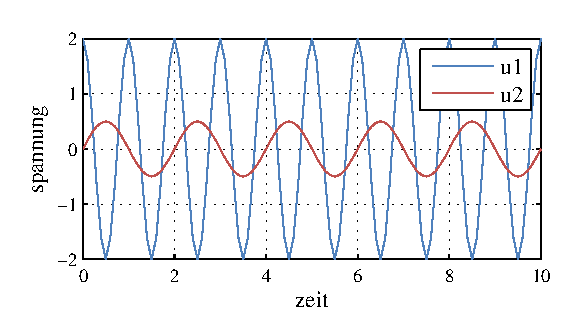
\includegraphics{./graphics/spannung}
  \caption{Verlauf der Spannungen $u_1$ und $u_2$.}
  \label{fig:sinus}
\end{figure}


\section{Formeln}

Eine einfache Formel:
\begin{equation}\label{eq:Test}
	q_3 = A_3 \alpha_3 \sqrt{\frac{2}{\rho}} \sqrt{p_3 - p_T}
\end{equation}

Eine Formel ohne Nummerierung:
\begin{equation*}
	u = - \frac{\partial \Psi}{\partial t}
\end{equation*}

\begin{eqnarray}
  \label{eq:system}
  \dot{\bvec{x}}&=&\mat{A}\bvec{x}+\bvec{g}(\bvec{x})u\\
y&=&\bvec{c}^{T}\bvec{x} + d u
\end{eqnarray}
Ein Verweis auf Gleichung \eqref{eq:system}.


\section{Abk�rzungen}

Vektoren sollten mit dem Befehl \verb+\bvec{}+ und Matrizen mit dem Befehl \verb+\mat{}+ gesetzt werden.

Abk�rzungen wie \eg, \ie, \zB, \dh, \sog, \ua, \bzw, \usw k�nnen mit den
Befehlen \verb+\eg+, \verb+\ie+, \verb+\zB+, \verb+\dh+, \verb+\sog+,
\verb+\ua+, \verb+\bzw+, \verb+\usw+ eingef�gt werden. Damit ergeben sich automatisch die richtigen Abst�nde vor und nach den Abk�rzungen.
